%&tex
\documentclass{standalone}

\usepackage[dvipsnames]{xcolor}

\usepackage{tikz}
\usetikzlibrary{positioning}

\begin{document}

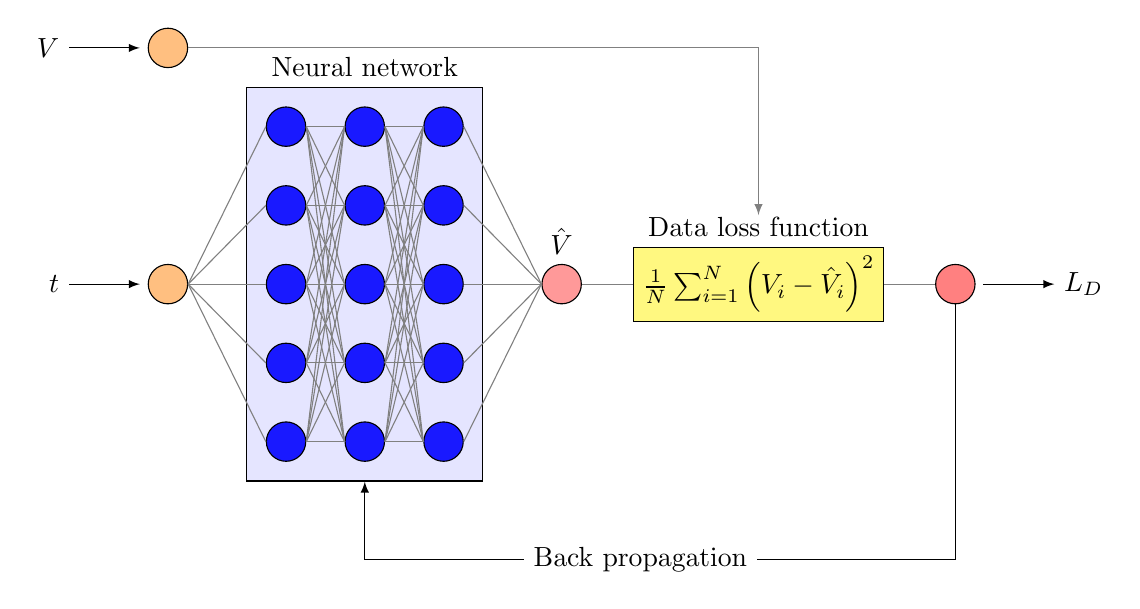
\begin{tikzpicture}
    % input layer node
    \node[draw,
    circle,
    minimum size = 0.5cm,
    fill=orange!50] (x) at (0,-0) {};

    % secondary input nodes
    \node[draw,
    circle,
    minimum size = 0.5 cm,
    fill=orange!50] (y_inp) at (0,3){};

    % hidden layer cover
    \node[draw,
    rectangle,
    minimum width = 3 cm,
    minimum height = 5 cm,
    label = Neural network,
    fill=blue!10] (HiddenLayerRectangle) at (2.5,0){};

    % hidden layer neurons
    \foreach \i in {1,...,5}
    {
        \node[draw,
        circle,
        minimum size = 0.5 cm,
        fill=blue!90] (HL_CL_1-\i)  at (1.5, \i-3.0){};
    }

    \foreach \i in {1,...,5}
    {
        \node[draw,
        circle,
        minimum size = 0.5 cm,
        fill=blue!90] (HL_CL_2-\i)  at (2.5, \i-3.0){};
    }

    \foreach \i in {1,...,5}
    {
        \node[draw,
        circle,
        minimum size = 0.5 cm,
        fill=blue!90] (HL_CL_3-\i)  at (3.5, \i-3.0){};
    }

    % output nodes
    \node[draw,
    circle,
    minimum size = 0.5 cm,
    label = \(\hat{V}\),
    fill=red!40] (y_pred) at (5.0,0.0){};

    % data function box
    \node[draw,
    rectangle,
    minimum width = 1 cm,
    minimum height = 0.5 cm,
    label = Data loss function,
    fill=yellow!50] (DataBox) at (7.5,0){\(\frac{1}{N}\sum_{i=1}^{N} \left(V_i - \hat{V}_i\right)^2\)};

    % Data loss node
    \node[draw,
    circle,
    minimum size = 0.5cm,
    fill=red!50] (y_Data_Res) at (10.0,0.0){};

    drawing connectors
    \foreach \j in {1,...,5}
    {
        \draw[color=black!50] (x.east) -- (HL_CL_1-\j.west);
    }

    \foreach \i in {1,...,5}
    {
        \foreach \j in {1,...,5}
        {
            \draw[color=black!50] (HL_CL_1-\i.east) -- (HL_CL_2-\j.west);
        }
    }

    \foreach \i in {1,...,5}
    {
        \foreach \j in {1,...,5}
        {
            \draw[color=black!50] (HL_CL_2-\i.east) -- (HL_CL_3-\j.west);
        }
    }

    \foreach \i in {1,...,5}
    {
        \draw[color=black!50] (HL_CL_3-\i.east) -- (y_pred.west);
    }

    \draw[color=black!50] (y_pred.east) -- (DataBox.west);
    \draw[color=black!50] (DataBox.east) -- (y_Data_Res.west);
    \draw[-latex,color=black!50, shorten >= 4mm] (y_inp.east) -| (DataBox.north);

    % labeling inputs and outputs
    \draw[latex-, shorten <= 1mm] (x.west) -- ++(-1,0) node[left]{\(t\)};
    \draw[latex-, shorten <= 1mm] (y_inp.west) -- ++(-1,0) node[left]{\(V\)};
    \draw[-latex, shorten <= 1mm] (y_Data_Res.east) -- ++(1,0) node[right]{\(L_{D}\)};

    % backpropagation sketch
    \node[below of = DataBox, yshift = -2.5cm, xshift = -1.5cm] (BP) {Back propagation};
    \draw[color=black] (y_Data_Res.south) |- (BP.east);
    \draw[-latex,color=black] (BP.west) -| (HiddenLayerRectangle.south);

\end{tikzpicture}

\end{document}
